\chapter{Introduction}
Particle Physics or sometimes called High Energy Physics, 
%\Jnote{No need to put colon in math mode. Also: This colon (and thepreceding clause) is not grammatical.}
is the field of physics that pursues the ultimate structure of matter, this is 
%\Jnote{is}
possible in two ways, one is to look for elementary particles, the ultimate constituents of matter at their smallest scale and the other is to clarify what interactions are acting among them
 \emph{(forces)}
%\Jnote{Never use math mode to change font of text. Probably you want something like \textbackslash emph\{\} here.}
to construct matter as we see it.

In our current view, all matter is made of three kind of elementary particles, \emph{leptons}, \emph{quarks} and \emph{mediators}.

Leptons have spin $\frac{1}{2}$, they naturally fall into three families, these are electron, muon, tau and their associated neutral neutrinos, those are described by lepton numbers for the example the electron has electron number 1 and the muon has electron number 0 and muon number 1 and so on. The three charged leptons have electric  charge -1. There are also six anti leptons for example the positron which has electron number of -1 and electric charge +1, so all in all we have 12 leptons.

The quarks have spin $\frac{1}{2}$ too, there are six flavours of quarks, up, down, top, bottom, charm and strange, quarks have a colour charge, which is property that is related to the strong interactions,  as the leptons there are also six anti quarks, we will talk about them in more details in following sections. 

Every interaction has its mediators, the photon for electromagnetic interactions, the gluon for the strong interactions, the two W' and Z for the weak interactions, and presumably the graviton for gravity.            
%\Jnote{There are a couple of grammatical mistakes in this sentence. Also,it is very long.}
 
There are four forces in nature, gravity, electromagnetism, weak nuclear force and strong nuclear force. In this essay our work will be on the strong nuclear force. 

\section{Quarks}
Quarks and leptons are the building blocks which build up matter. As mentioned above
%\Jnote{In the present?}
there are six "flavours" of quarks, these are up, down charm strange, top and bottom.
%\Jnote{s/can written/can be written}
%\begin{equation*}
%  \left( \begin{array}{c}          
%           \text{up}\\
%          \text{down}\\
%         \end{array}
%  \right);  \hspace{1cm}    
%  \left (\begin{array}{c}
%           \text{charm}\\
%           \text{strange}\\
%         \end{array}
%  \right)  ;  \hspace{1cm} 
%  \left( \begin{array}{c}
%           \text{top}\\
%           \text{bottom}\\
%         \end{array}
%  \right)
%\end{equation*}  
%\Jnote{What do you mean they can be written like that? What those matrices
%  (vectors?) mean?}
Quarks can successfully account
%\Jnote{s/a count/account}
for all known mesons and baryon which are known as hadrons, which are particles with spin $\frac{1}{2}$. Mesons consist
%\Jnote{s/are consist/consist}
of quark and anti quark for example the positive pion $\pi^+$ which consists of up and anti down quarks. Baryons consist of three quarks or three anti quarks for example the proton which consists of two up quarks and one down quark.
%\Jnote{Maybe give examples of mesons and baryons?}

Quarks carry colour quantum number: red, green or blue, the colour name here is an analogy  that is famously used among physicists to describe a three kind of generating force, we may call them by a number or any other index, also we can think of it as a three primary additive colours. Since all hadrons are colour charge neutral or colourless particles they have white charge. 
%\Jnote{What is the meaning of white charge? How does it compare to other
%  colors?}

Unlike other elementary particles quarks carry fractional charge and possess new quantum numbers.
%\Jnote{s/posses/possess}
%\Jnote{What is quantum number?}
The table \ref{table1.1} summarizes
%\Jnote{s/summarize/summarizes}
some properties of quarks.
Each quark flavour is associated with its own quantum number\footnote{These are the set of numbers that describes a conserved quantities in the dynamic of a quantum system, for example the set of numerical solutions of Schrödinger equation of the Hydrogen atom.}(the capital letters), those quantum numbers describes the decay of the particles, those first were meant to explain the fact that some particles decay slower than other particles, for example the first mentioned below the "Strangeness", it has been noticed that the higher the mass the lower the strangeness,  these numbers are conserved in strong and electromagnetic interactions but not in weak interaction, 
These are: 
\begin{itemize}
\item[•]Strangeness: $S=-1$ for s-quark.

\item[•]Charm: $C=+1$ for c-quark.

\item[•]Beauty: $\tilde{B}=-1$ for b-quark. 

\item[•] t - quark has life time too short to form hadrons. 
\item[•]up and down quarks have nameless flavour quantum numbers.
\end{itemize} \citep{particle}
%\Jnote{What exactly is conserved here? Are these six values or just one?} 

\begin{table}
\begin{center} 
 \begin{tabular}{|c|c|c|c|} \hline 
  Name (Flavour) & Symbol & Electric charge(in units of e) & Mass  \\ \hline 
  $\text{Up}$ & $\text{u}$ &$ +\frac{2}{3}$ & $1.7-3.1 \frac{Mev}{c^2}$\\\hline
  $\text{Down}$&$\text{d}$&$-\frac{1}{3}$& $4.1-5.7\frac{Mev}{c^2}$\\\hline
  $\text{charm}$&$\text{c}$&$+\frac{2}{3}$&$1.18-1.34\frac{Gev}{c^2}$\\\hline
  $\text{strange}$&$\text{s}$&$-\frac{1}{3}$&$80-130\frac{Mev}{c^2}$\\\hline
  $\text{top}$&$\text{t}$&$+\frac{2}{3}$&$172.3-173.5\frac{Gev}{c^2}$\\\hline
  $\text{bottom}$&$\text{b}$&$-\frac{1}{3}$&$4.13-4.37\frac{Gev}{c^2}$\\\hline
 \end{tabular}
\caption{properties of Quarks}
\label{table1.1}
\end{center}
\end{table}

%\Jnote{Maybe extend the table to explain other properties of quarks?}

\Jnote{Citations: If section(s) are based on a textbook, cite it in
  the beginning, saying something like ``the following
  presentation is based on \textbackslash cite\{...\}''}

\section{Strong Force}
As we mentioned the elementary particles that mediate these interactions
%\Jnote{''this interaction'' or ''these interactions''}
are eight called gluons, which come from the gauge group $SU(3)$ which has eight generators, gluons mediate the interaction between quarks.


%\Jnote{This is a thesis, not a research paper. Therefore, it needs to have
%  an expository part. You shouldn't throw around terms like ``gauge bosons'',
%  ``gauge group'' or even ``gluons'' and ``quarks'' without some introduction.
%  Think of it like this: Dedan should be able to understand
 % the first three pages of your thesis.}

%\Jnote{In particular, I think it would be helpful if you explained
%  relations between all the particle names (hadrons, gluons, leptons,
 % quarks, bosons etc.)}

Gluon is massless spin $1$ particle, carrying charge called colour charges, gluons
%\Jnote{s/glouns/gluons (here and elswhere)}
look like photons but photons do not carry electric charge,
%\Jnote{Is colour charge the same as electric charge? It is not clear to me from this sentence.}
because of that gluons can interact among themselves unlike photons.
Normally the range of the force can be calculated by a
simple argument of the uncertainty\footnote{$\Delta E \Delta t \approx m c^2 \Delta t > \frac{\hbar}{2} \Longrightarrow range = c \Delta t > \frac{\hbar}{2 m c}$},
%\Jnote{What is ``argument of uncertainty''? Do you mean uncertainty principle
 % or something else?}
but this not the case for the strong force, the strong force is more complicated
and involves a concept known as confinement.

The colour charge has strange property that it exerts a constant force that binds colour carrying particles together, this can be visualized using the analogy of a rubber band, the stronger you pull on the rubber band the tighter it feels.
If we do not pull on it at all, it hangs loose.
%\Jnote{s/hang/hangs}
%\Jnote{It is not usual to address the reader %in 2nd person in research texts.
%3rd person or passive voice are more common. %Personally I don't think it's
%a big deal, though.}
The same thing happens for the particles,  that means at a very short distance, the force is relaxed and the particles behave as free particles,
%\Jnote{s/a free particles/free particles}
as the distance between them increases the force acts
%\Jnote{s/act/acts}
like a rubber band, the force gets
%\Jnote{s/get/gets}
them back in stronger pulling
%\Jnote{You got lost in the grammar somewhere around this point.}
and when the rubber band is stretched beyond its limits then it will cut into many pieces producing more particles.
%\Jnote{Future tense at the end is inconsistent with the rest of the sentence.}
%\Jnote{Another long sentence. Consider dividing it into simpler parts.}
This phenomenon is known as the colour confinement. In other words those particles
%\Jnote{s/particle/particles}
tend not to be
%\Jnote{s/not be/not to be}
separated by a macroscopic distance.
%\Jnote{What about when the rubber band ''breaks''? Can the macroscopic distance be achieved then?}
This limits the range of strong force, which is believed to be on order of $10^{-15}\si{m}$,
%\Jnote{Google ''siunitx'' to see how to write units in Latex.}
the dimension of a nuclear particle.

The theory which describes this force is called $Quantum$ $Chromodynamics$.
\Jnote{Citation for this section would be nice.}

\section{Large Hadron Collider}

Hadron colliders are devices made to explore the world of particle physics, they work as theories testers and also as a discovery machines, an example of these hadron Colliders is the LHC in CERN.

In the Large hadron Collider
%\Jnote{Rule for capitalization: if given name, capitalize (almost) all words,
%  otherwise don't capitalize. So, ``hadron collider'' (as a type of device),
%  but ``Large Hadron Collider'' (the one at CERN).}
two beams of hadrons (protons)
%\Jnote{Put space before opening bracket.}
are being accelerated to a high kinetic energy and then collided with each other. It has started operation in 2009 and in 2013 the Higgs particle has been discovered in LHC. Most of the interesting physics at LHC involves investigating the results of these interactions(collisions), as a result of this collision stable partons are formed, partons consists of quarks and qluons.

Because of the complex nature of the event at the hadrons colliders, the description of the final state involves a multi-particle calculations. The accurate prediction of the final state in hadron colliders is still one the hardest problems, this problem roots to the non-abelian nature of QCD, which leads to a colour confinement at a long distances. The two main problems are the description of the hadron formation and the evolution of QCD final states from short to long distances. Those problems can be tackled to a good approximation by Monte-Carlo event generators.

%\Jnote{Consider splitting text above into paragraphs.}

\section{The Parton Shower}
In general parton showers are approximations of the higher order real emission corrections(this refers to the stable hadrons) to the hard scattering. The word "hard" here means,
%\Jnote{Put ``hard'' in quotes.}
the process involves a transfer of large momentum, either a violent scatter or creation of large mass. They locally conserve flavour and four momentum, and also they are consistent, which means, the particle either splits into two or not. 
Since the parton showers are simulate of the branching and splitting processes, the quality of their predictions depend on precise is the implementation, for example one can ensure the colour coherence through selecting an evolution variable representing the angular ordering, although, this in not the only choice to ensure the colour coherence \citep{introduction}.
%\Jnote{``higher order real emission corrections'', ``evolution variable representing the angular ordering'', don't use lots of complicated words without explaining them.}
In the following we will at a simple implementation of a parton shower in python.

\section{Hadronization}  

To reflect the colour neutrality of the particles in our model the partons will be transformed into a stable hadrons which are colour neutral, this process is called hadronization. The first implemented model and also follows Monte-Carlo event generators was Feynman-Field Model, which gives an idea of the formation of the mesons through iteratively from a single quark. However, this model is not collinear safe,
%\Jnote{Explain what ``collinear safe'' means.}
which means the model can mix the short and long distance physics. Now a days two models are common, the string model and clustering model\citep{introduction}. 
     
      
\section{Monte Carlo Method}
The name Monte Carlo method is set of mathematical tools that first used by scientist working on the nuclear project in Los Alamos. The essence of the is to generate numbers with probability that can be used to study physical phenomena. In our context the definition of Monte Carlo method would be, that in which we use randomly generated numbers to imitate a physical behaviour that is not necessarily considered to be random \citep{montecarlo}.
%\Jnote{I did not understand any of the two sentences above.}

\subsection{Pseudo-random numbers}
In a computer these are generated using a deterministic algorithm that generates a set of numbers that exhibits statistical randomness, those numbers are called pseudo-random \citep{montecarlo}.
%
%The main properties of a good random generator are:
%
%\begin{itemize}
%\item[•]\textbf{Long period}: the pseudo-random generators have a finite range after which they begin to repeat themselves, for a good random generator this range should much longer than the amount of numbers that are needed for the calculation. 
%
%\item[•]\textbf{Randomness}: The numbers should follow the uniform distribution and also should be independent of each other.
%  \Jnote{This is not correct. Pseudo-random numbers are, by definition,
%    determinstic (so not random). What you want is that they ``look like''
%    i.i.d.~uniform random numbers in all important respects
%    (where ``important'' is not well-defined and depends on what
%    exactly you are doing).}
%
%\item[•]\textbf{Repeatability}: The same initial values should give the same sequence of a random numbers, this important for testing because one might need to repeat the calculation or in the coding terms debugging.
%
%\item[•]\textbf{Portability}: One should be able to generate the same sequence in different machines. 
%
%\item[•]\textbf{Fast}: the generation of the pseudo-random numbers should not be time consuming\citep{Weinzierl}.    
%\end{itemize}
%
%\Jnote{I don't think it is necessary that you dwell on pseudorandomness,
%but once you mentioned it, please explain how it connects to Monte Carlo.}


\subsection{Samples with different PDFs}

Generating samples of different probability distribution function(pdf) is essential since we are simulating various variables that have different numerical behaviour. For example if our pseudo-random numbers are uniformly\footnote{Uniform means that every value in the range of the distribution is equally likely to occur. This distribution is widely used for generating random numbers for other distributions, it is denoted by $U$.} distributed in the interval $[0,1]$  and instead we need numbers that have normal distribution restricted to the same interval. I will discuss two methods, which are used in this essay.
%\Jnote{Be clearer what you are trying to achieve. You want to sample from
  %given distribution provided you can sample from another distribution
  %(for example uniform over $[0, 1]$).}

\subsection{The acceptance-rejection method}

The acceptance-rejection method was developed by von Neumann \citep{Weinzierl}.
Assume we have access to a sample which is distributed according to the pdf $f(x)$,
and the let us denote the pdf of the required distribution by $p(x)$, we assume that for both $p(x)$ and $f(x)$ $x$ varies over a finite interval.
 
In simple words, first we generate $x$ according to the uniform distribution over a given interval assume $[0,1]$ 
, then we find the maximum of $f(x)$, and then calculates $p(x)$, then we generate another number $y$ which is also uniformly distributed over the interval $[0,f_{max}(x)]$, and checks  $y \times f(x) \leq p(x)$.
If this the case then accept $x$, if not reject $x$ and start again, example of that, if have a number $x$ that is fall under uniform distribution and we want to reshape this so that we get a number  that has the distribution $\frac{1}{x}$, then we find the maximum value of probability density function ($p(x)$) for $x$, here we add small number to $x$ so that we avoid the singular point when $x = 0$, after that we generate another sample $y$ that is also uniformly distributed in the interval $[0,pdf_{max}]$, 
now we check if $y $ is less than $p(x)$ we add $x$ to our distribution if not we start again. The histograms in figure \ref{Fig:2} demonstrate the example above.   
\begin{figure}
    \centering
    \begin{subfigure}[b]{0.5\textwidth}
        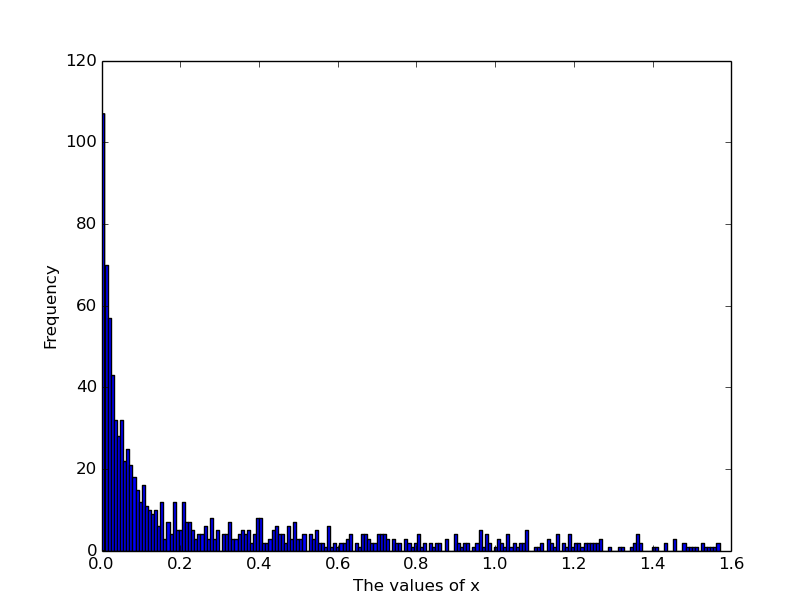
\includegraphics[width=\textwidth]{images/inverse_method.png}
        \caption{Theta values}
        \label{fig2}
    \end{subfigure}
    ~ %add desired spacing between images, e. g. ~, \quad, \qquad, \hfill etc. 
      %(or a blank line to force the subfigure onto a new line)
    \begin{subfigure}[b]{0.5\textwidth}
        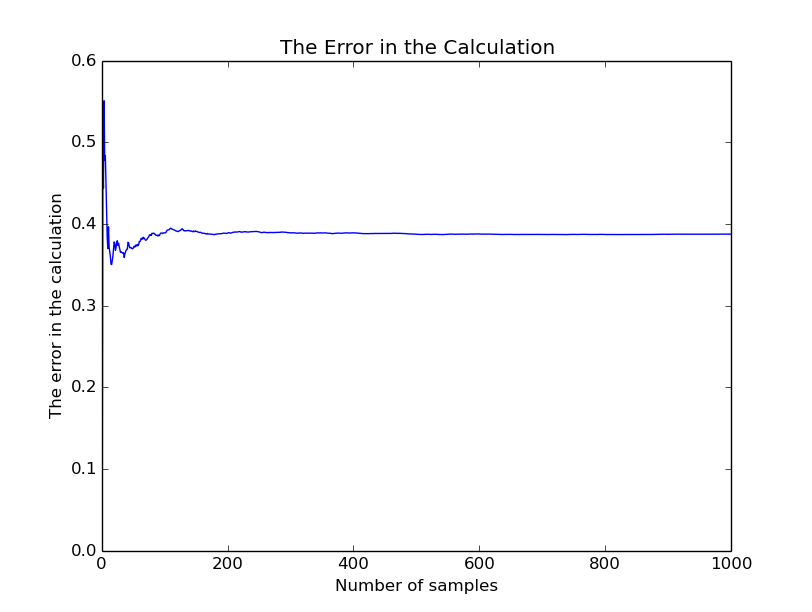
\includegraphics[width=\textwidth]{images/uncertainity_.png}
        \caption{The uncertainty}
        \label{fig2}
    \end{subfigure}
    \label{Fig:2}
\caption{}
\end{figure}

Another related example of this method is calculation of pi, assume we have a box of side length D and a circle of diameter D inside that box, now the probability that a point in the box and is also in the circle is approximately the area of the circle over the area of the box, which is $\pi$ over 4 here, hence, from this we can approximate the value of $\pi$. The histograms in Figure \ref{fig:1.1} exhibits this calculation and also the error in the calculation\citep{Weinzierl}.
%\Jnote{I wouldn't call it ``example'' of what you described before. It is a related thing, but an example should give specific$f$ and $p$.}


\begin{figure}
    \centering
    \begin{subfigure}[b]{0.5\textwidth}
        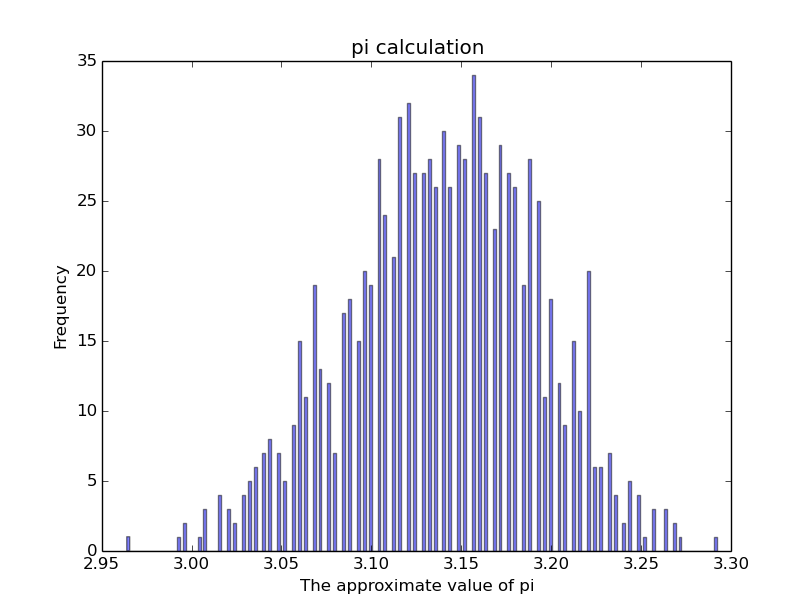
\includegraphics[scale=.5]{images/pi_value.png} 
        \caption{pi value}
        \label{fig:gull}
    \end{subfigure}
    ~ %add desired spacing between images, e. g. ~, \quad, \qquad, \hfill etc. 
      %(or a blank line to force the subfigure onto a new line)
    \begin{subfigure}[b]{0.5\textwidth}
        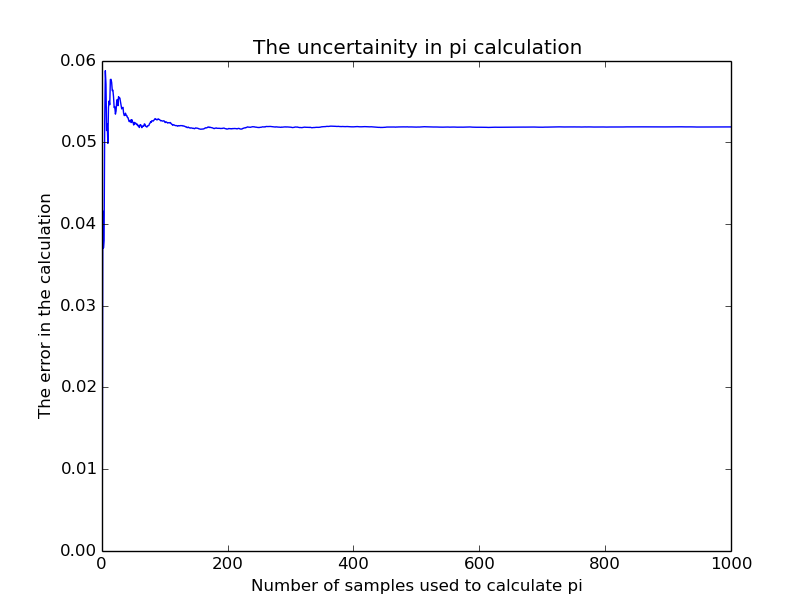
\includegraphics[scale=0.5]{images/uncertainity_pi.png}
        \caption{The uncertainty}
        \label{fig:tiger}
    \end{subfigure}
    \label{Fig:1}
\caption{At the top, this a histogram shows the values of $\pi$ that are generated from sampling 1000 numbers. At the bottom the plot shows the error in the calculation when we use different number of samples} 
\label{fig:1.1}
\end{figure}

%\Jnote{Consider giving a file name (files will be attached as appendix)
%whenever you are presenting a calculation, like with the histograms here.}


\subsection{The module random in python}

The samples above were generated using Python module \verb+random+, here are few words about this module.

%\Jnote{For module, variable and file names you can use verbatim command like this:
%\textbackslash verb+my\_file.py+}.
 
This module implements pseudo-random number generators for various distributions.

In a computer pseudo-random numbers are generated using a deterministic algorithm that generates a set of numbers that exhibits statistical randomness, those numbers are called pseudo-random.

For integers, there is uniform selection from a range. For sequences, there is uniform selection of a random element, a function to generate a random permutation of a list in-place, and a function for random sampling without replacement.

On the real line, there are functions to compute uniform, normal (Gaussian), lognormal, negative exponential, gamma, and beta distributions. For generating distributions of angles, the von Mises distribution is available.

Almost all module functions depend on the basic function random(), which generates a random float uniformly in the semi-open range $[0.0, 1.0)$. Python uses the Mersenne Twister as the core generator. It produces 53-bit precision floats and has a period of $2^{19937}-1$\citep{python}.


\section{Parton Shower Simulation}

The following is a simple simulation in python for a splitting of a single quark, the simulation accounts for the four momentum conservation of the soft particles.
\Jnote{Why only soft?}

\subsection{Physical description}
\noindent As a result of a hadrons collision, quarks will fly away. Since they are charged particles(colour charge), the moving quarks will radiate. The quark will lose part of its energy emitting a gluon. If at the beginning, the quark had energy $E_i$ and radiates energy $E_{rad}$, then the qluon takes $\frac{E_{rad}}{E_i}$ of the particle's initial energy.
\Jnote{You mean it takes $E_{rad}/E_i$ \emph{fraction} of initial energy.}
It is radiated at an angle of $\theta$ to the quark initial direction. The quark will fly on radiating another gluon and so on until it becomes stable(the hadronization starts).
\Jnote{Put space before opening parenthesis (here and elsewhere).}
The radiated gluons will decay into two quarks, which will later radiates gluons,  which will radiate gluons again and so on. The result is a shower of partons decaying into two partons. 
\begin{figure}[hbtp]
%\caption{}
\centering
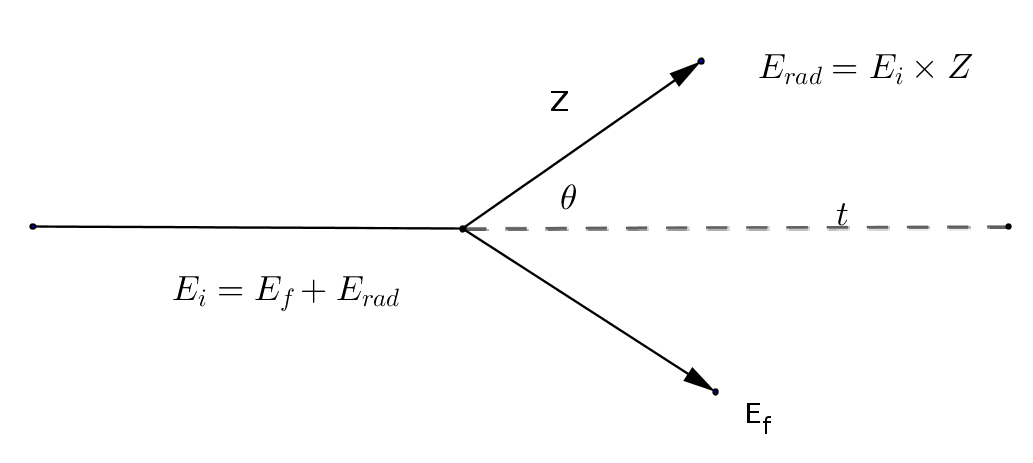
\includegraphics[scale=.3]{images/tt.png}
\caption{The splitting of a particle into two particles}
\end{figure}

\Jnote{You need to make clear that in your model you do not make distinction
  between quarks and gluons.}

\Jnote{The picture with collision is way too small. Also caption is missing.}

Now we begin with 4- momentum vector \begin{equation}
P^{\mu} = \begin{pmatrix}
E/c& \\p_x&\\ p_y &\\ p_z 
\end{pmatrix}
; 
P_{\mu} = \begin{pmatrix}
E/c& \\-p_x&\\-p_y &\\ -p_z 
\end{pmatrix}
\end{equation}   And the inner product is given by \begin{equation}
P^{\mu} P_{\mu} = P^{\mu} \eta_{\mu \nu} P_{\nu} =  (m_0 c)^2 
\end{equation} \begin{equation} P^{\mu} P_{\mu} = \left(\frac{E}{c}\right)^2 - (p_x^2 + p_y^2 + p_z^2) = (m_0 c)^2 \end{equation} Now considering the natural units $c =1$ this can be written as \begin{equation}\label{4} m_0^2 = E^2 - \Vert p \Vert \end{equation} Which is lorentz invariant quantity i.e does not depend on the frame. In our case the quarks in (LHC), the mass of the quark $\sim$ 1 Mev and the energy of the hadrons is $\sim$ 1 Tev, hence, we can assume that the mass of the quark(\ref{4}) is $0$.

From the conservation of energy and momentum, \Jnote{Don't put blank line
  before the equation here.}

\begin{equation}
P_{i}^{\mu} = P_f^{\mu}.
\end{equation} 
We assume that the intial patricle is moving in x -direction, we can write the initial 4-momentum as $P_i^{\mu} = (E,E,0,0)$, afterwards the particle will split. Therefore, the final momentum is given by $P_{rad} + P_{part}$, part here refers to the particle which has lost part of its energy, so $P_{rad} = (E_{rad},\  cos\theta \cdot E_{rad},\  sin\theta \cdot E_{rad},\ 0)$. From this, and since the particle is rotated with $\theta$ we can find the direction of the particle(part) with help of the rotation matrix
\Jnote{Please make clear that the other particle will have non-zero mass.}
\begin{equation} R = 
\begin{pmatrix}
\cos\theta & - sin\theta\\
\sin\theta & \cos\theta
\end{pmatrix}
\end{equation} The direction of the particle of the fraction enregy can be found using the following equation  \begin{equation}
P_{part} = P_{i} - P_{rad} .
\end{equation}    
In a three dimensional world, we have two rotation angles, the angular angle and the azimuthal angle. Given a unit vector $u =(u_x, u_y, u_z) $, where $u_x^2 + u_y^2 + u_z^2 = 1$,the matrix for rotating this particle by angle $\theta$ about an axis in the direction of $u$ is   
\begin{equation} 
\begin{pmatrix}
\cos\theta + u^2_x(1-\cos\theta) & u_x u_y (1-\cos\theta) - u_z \sin\theta& u_x u_z(1-\cos\theta)+ u_y \sin\theta\\

u_y u_x (1 - \cos\theta) + u_z \sin\theta & \cos\theta + u_y^2 (1 - \cos\theta) & u_y u_z (1 - \cos\theta) - u_x \sin\theta \\

u_z u_x (1 - \cos\theta) - u_y \sin\theta & u_z u_y (1 - cos\theta) + u_x \sin\theta & \cos\theta + u_z^2 (1 - \cos\theta)
\end{pmatrix}
\end{equation}

\Jnote{OK, but you have to explain 3D case in detail. Consider making separate
  sections for 2D and 3D. Picture showing what is angular (is this
  correct name?) and azimuthal angle would be helpful.}

\subsection{Implementation in python}
First we will start with case of 2 dimensions model which accounts for one rotation matrix $\theta$ and it evolves generation of two random numbers, one them represent the angle and the other regards the energy of the radiated particle. Here both the energy fraction $z$ and the angle $\theta$are following the distribution $1/x$, where the former lies in the interval [0.25, .75]
\Jnote{No, it does not lie in $[0.25, 0.75]$. Give the correct distribution.
  Also mention the cutoff values you are using (to avoid singularity at $x=0$).}
\Jnote{Put all of numeric intervals in math mode.}
and the later in the interval [0,$\pi/2$] and they are generated by applying the inverse transform method on a set of numbers that are uniformly distributed.

As for the four momentum vector, the module $numpy$ is used for this purpose, here we use the object $array$. \verb+Numpy+ is a scientific computing package in python which is widely used for these purposes, beside that it has powerful N-dimensional arrays it also has useful linear algebra tools and random number capabilities.         

following the physical description a list contains the four momentum of the initial particle was defined, then we assumed that the particle has initial energy = 1 energy unit, since the particle will split after certain distance an assumption of the distance before the decay was made is that the particle will move a distance of 1 unit and then it will decay, basically it is an iteration process,  at the beginning we check the energy of the particle if it is a above the stability limit, which we assumed to $0.09$, this particle will split, the direction of the radiated will follow the $\theta$ and its energy will be given from $z$, and then both new particles four momenta will be add to the list at the beginning and again those particles will be checked, now if the particle has energy that is equal or below the stability limit then the iteration process will be terminated.   

As for plotting the results, the library $matplotlib$ was used which is a library that is used to make 2 D plots in Python, as $matplotlib$ has the ability to add many lines at once, here the Linecollection is used, which is a package in $matplotlib$, the diagram in figure 3 shows the 2 D simulation of the parton shower.  \begin{figure}[H]
\centering
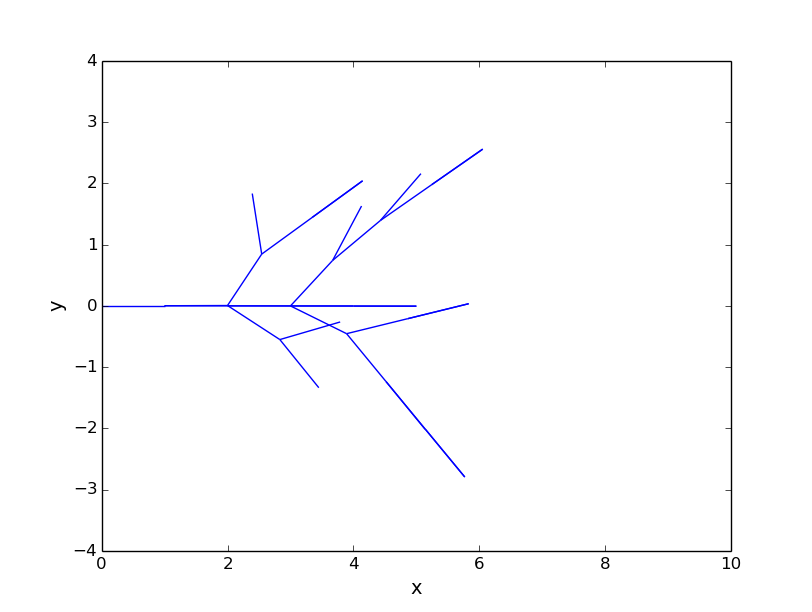
\includegraphics[scale=.5]{images/2D_partonshower.png}
\caption{2D simulation of the spliting of a single parton, here the colour fades as the energy decreases}
\end{figure}

The 3D simulation of the parton shower is essentially the same as for python code with few changes, in which now we have two rotation angles, $\theta$ and also $\phi$ which is the azimuthal angle which is uniformly distributed in the interval [0,2$\pi$]. To simulate the rotation in three dimensions, the function \verb+normv(u)+ and function \verb!rotation(v,angle)!, the former returns the axis of the rotation, the function input and the vector [1,1,1] from a plane, from which we find a vector that is orthogonal to this plane, and the later is matrix of rotation, it takes the angle rotation and the axis of rotation as inputs. 

Also here z (the energy fraction) now is lies the interval[0,1] and the stability limit is 0.05. The digram in figure 4 shows the 3D simulation of single parton splitting.

\Jnote{This description (both 2D and 3D case) should be way longer,
  more organized and more detailed. It should take several pages and you
  should explain what the code is doing precisely and in detail.}
 
 \begin{figure}[H]
\centering
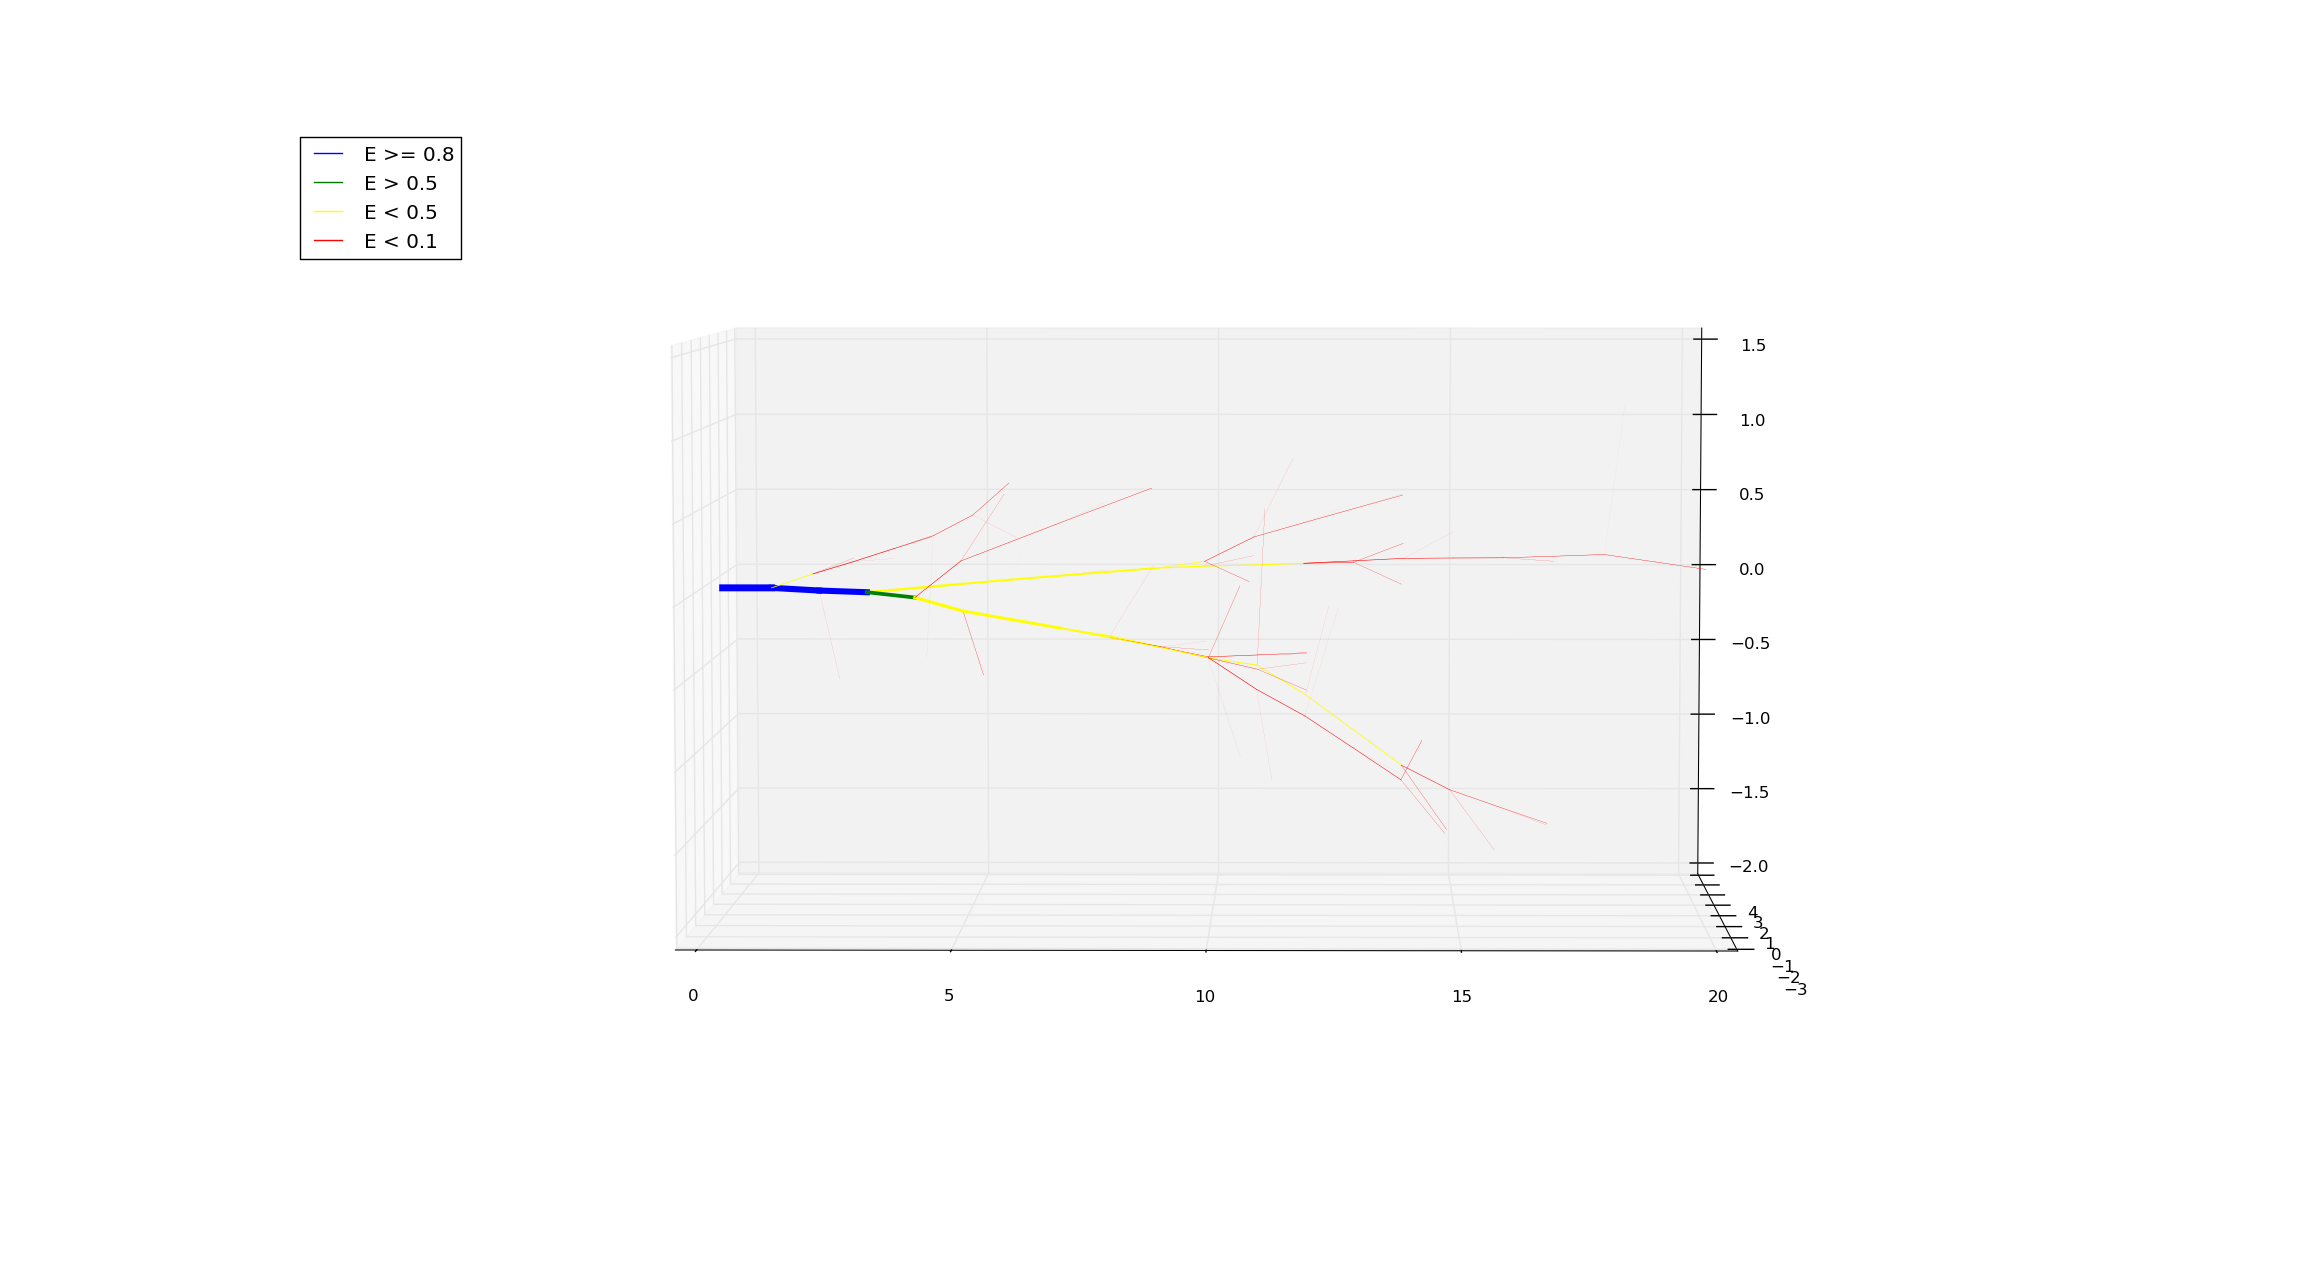
\includegraphics[scale=.3]{images/3D_partonshower.png}
\caption{3D simulation of the spliting of a single parton}
\end{figure}
